\section{Methodology}
\label{sec:tist_methodology}

Consider a labeled source dataset, $\mathcal{S}$, with training images $\mathcal{X_S}$ and corresponding segmentation labels $\mathcal{Y_S}$, while we denote a target dataset $\mathcal{T}$, containing only target images $\mathcal{X_T}$. We aim to train a network using $\mathcal{X_S}$, $\mathcal{Y_S}$, and $\mathcal{X_T}$ for semantic segmentation in the target dataset. 

We propose to train the model using a self-supervised approach on the images $\mathcal{X_T}$ by assigning pseudo labels during training. Typical pseudo labels are computed from independent predictions of unlabeled images. Instead, our proposed framework adopts a self-assessment strategy to determine the reliability of predictions in an unsupervised fashion. Specifically, we propose to target highly reliable predictions generated by a network aiming for transformation-invariant confidence. Compared to self-ensembling strategies that penalize the distant predictions corresponding to the transformed versions of identical inputs, our goal is to filter out transformation-variant predictions. Indeed, our method reinforces the ensemble of high-confidence predictions from two versions of the same target sample. The proposed TI-ST framework simultaneously trains on the source and target domains to progressively bridge the intra-domain distribution gap. \Cref{fig:tist_method} depicts our TI-ST framework, which we detail in the following sections. 

%\begin{figure}[t]
%\centering
%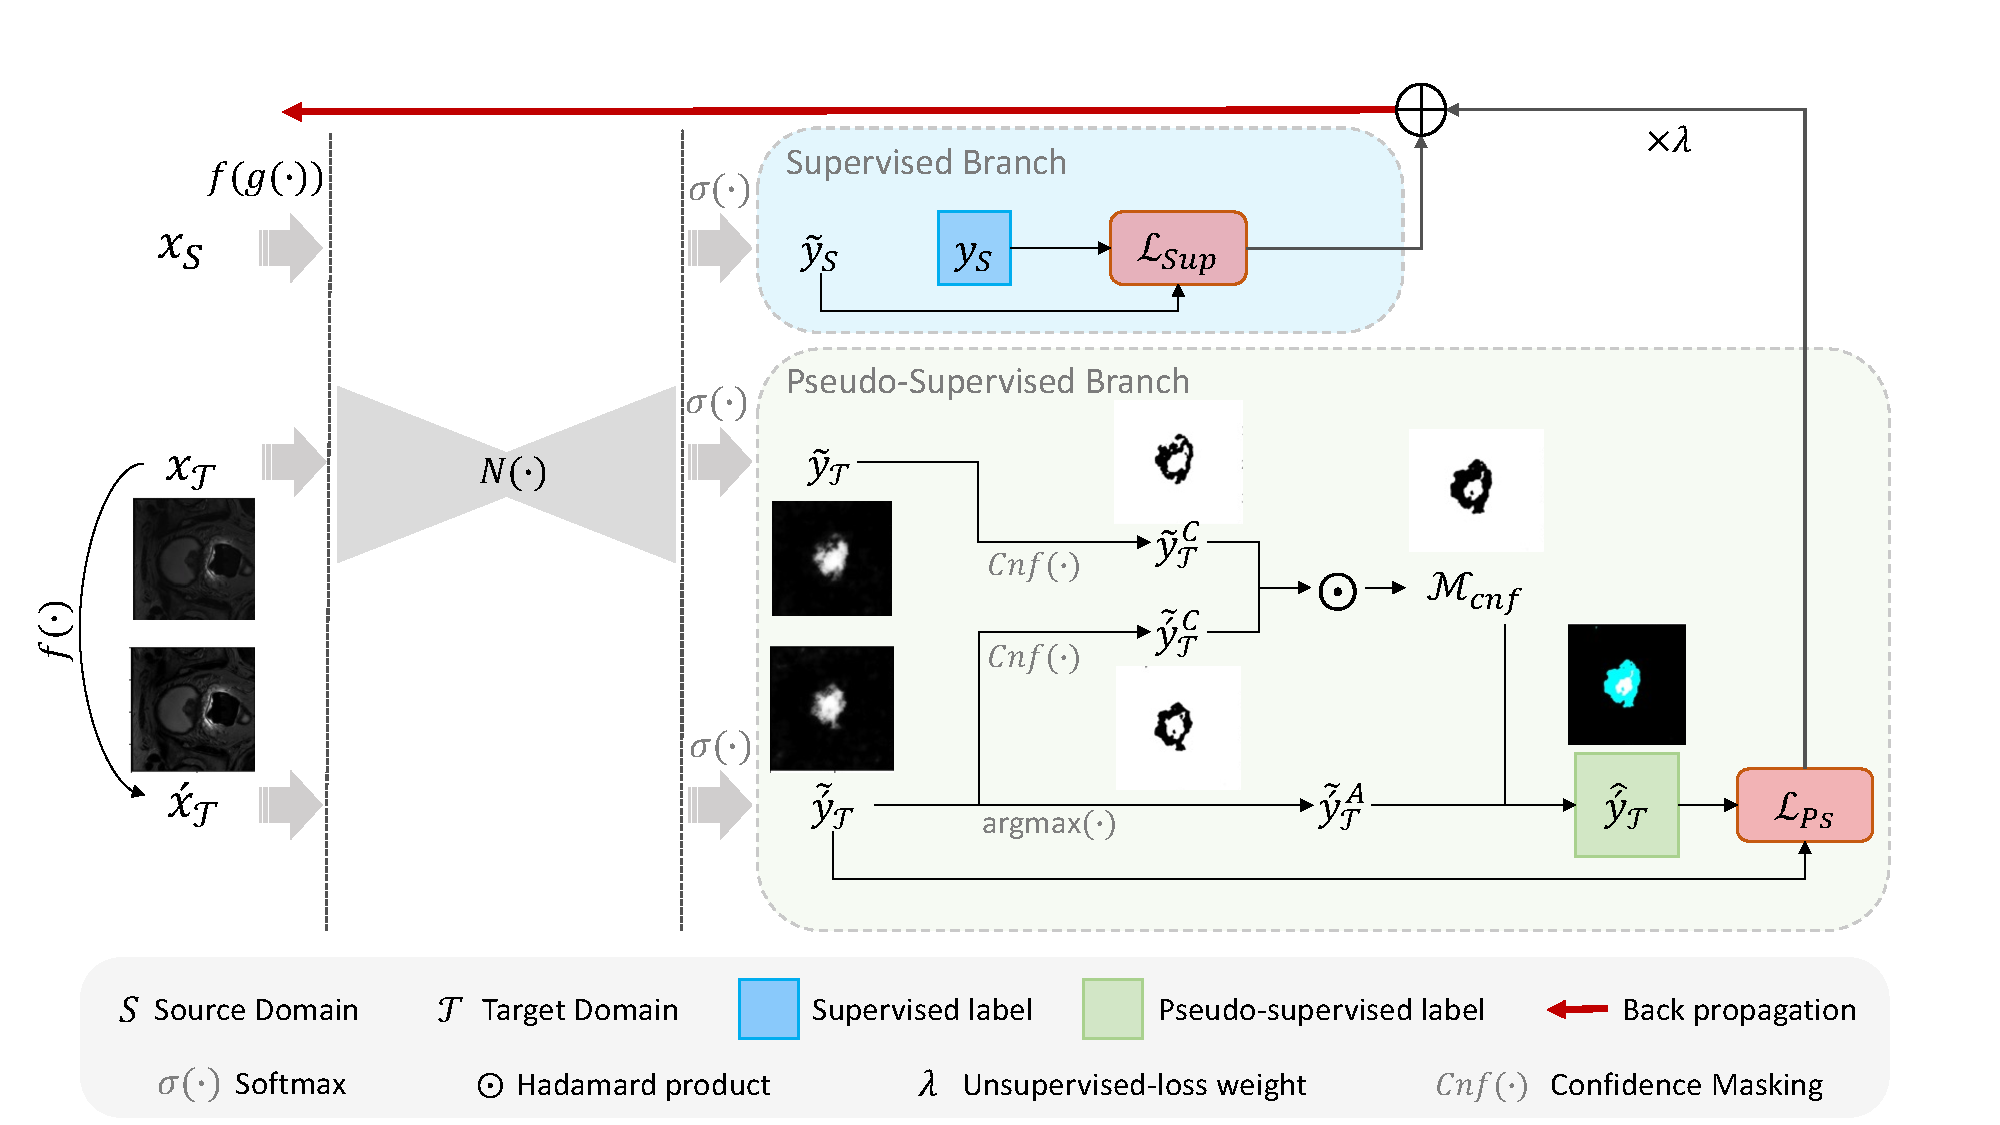
\includegraphics[width=\textwidth]{figures/BD8.pdf}
%\caption{Proposed unsupervised domain adaptation framework based on transformation-invariant self-training (TI-ST). Ignored pseudo-labels during unsupervised loss computation are shown in turquoise.
%}
%\label{fig:BD}
%\end{figure}

\textfig[t]{1}{figures/tist_method.pdf}{Proposed unsupervised domain adaptation framework based on transformation-invariant self-training (TI-ST). Target images $\x_\mathcal{T}$ and their non-spatially transformed pairs $\x'_\mathcal{T}$ are fed to the network $N$ to produce $\y_\mathcal{T}$ and $\y'_\mathcal{T}$. A confidence-mask ensemble is built from the corresponding segmentations, and this is compared to $\y'_\mathcal{T}$ in the pseudo-supervised loss $\mathcal{L}_{Ps}$.}{fig:tist_method}

\subsection{Model} 
At training time, images from the source dataset are augmented using spatial $g(\cdot)$ and non-spatial $f(\cdot)$ transformations and passed through a segmentation network, $N(\cdot)$. At the same time, images from the target dataset are also passed to the network. Specifically, we feed two versions of each target image to the network: (1) the original target image $\x_\mathcal{T}$, and (2) its non-spatially transformed version, $\x'_\mathcal{T} = f(\x_\mathcal{T})$. Once fed through the network, the corresponding segmentations can be defined as $\tilde{\y}_{\mathcal{T}} = \sigma(N(\x_{\mathcal{T}}))$ and $\tilde{\y}'_{\mathcal{T}} = \sigma(N(\x'_{\mathcal{T}}))$, where $\sigma(\cdot)$ is the Softmax operation. The segmentations correspond, therefore, to the probability of each pixel to be classified as foreground or background\sidenote{Hence, $\tilde{\y}_{\mathcal{T}}\in [0,1]^{C\times W\times H}$ and the same applies to $\tilde{\y}'_{\mathcal{T}}$. $C$ represents the number of classes, and $W$ and $H$ are the width and height of the initial image, respectively.}. We then define a confidence-mask ensemble as
\begin{equation}
\mathcal{M} = \text{Cnf}~(\tilde{\y}_{\mathcal{T}}) \odot \text{Cnf}~(\tilde{\y}'_{\mathcal{T}}),
\label{eq:ensemble_confidence}
\end{equation}
where $\odot$ refers to Hadamard product used for element-wise multiplication, and $\text{Cnf} \in \{0, 1\}^{W\times H}$ is the high-confidence masking function with a confidence threshold $\tau$. For pixel $(i,j)$, this takes the form:
\begin{equation}
    \text{Cnf}_{(i,j)}(y(i,j)) =
    \begin{cases}
        1, & \text{if    } \max_c(\y(i,j)) > \tau\\
        0, & \text{otherwise  }
    \end{cases}
    \label{eq:filtering}
\end{equation}

$\mathcal{M}$ encodes regions of confident predictions invariant to transformations. Finally, we can compute the pseudo-ground-truth mask for each input from the target dataset as
\begin{equation}
\hat{\y}'_{\mathcal{T}} = 
    \begin{cases}
        \argmaxH_{\textsub{C}} (\tilde{\y}'_{\mathcal{T}}), & \text{if  } \:\mathcal{M} = 1\\
        \text{ignore}, & \text{otherwise}
    \end{cases}
\end{equation}

\Cref{tab:tist_var_list} summarizes the variables that the method uses.

\subsection{Training}
To train our model, we simultaneously consider both the source and target samples by minimizing the following loss,
\begin{equation}
    \mathcal{L} = \mathcal{L}_{Sup}( \tilde{\y}_\mathcal{S}, \y_\mathcal{S}) + \lambda \mathcal{L}_{Ps}(\tilde{\y}'_{\mathcal{T}}, \hat{\y}'_{\mathcal{T}}),
    \label{eq: loss}
\end{equation}
\noindent
where $\mathcal{L}_{Sup}$ and $\mathcal{L}_{Ps}$ indicate the supervised and pseudo-supervised loss functions respectively. We set $\lambda$ as a time-dependent weighing function that gradually increases the share of pseudo-supervised loss. Intuitively, our pseudo-supervised loss enforces predictions on transformation-invariant, highly-confident regions for unlabeled images. 

\begin{margintable}[]\small
\caption{List of variables and their description}
\label{tab:var_list_loc}
\begin{tabular}{@{}cl@{}}
\toprule
\textbf{Var.}       & \textbf{Description}                                                                                         \\ \midrule
$H$            & Slice height                                                                              \\
$W$            & Slice width                                                                           \\
$C$            & Num. of columns                                              \\
$\x$           & 2D OCT slice                                                                                        \\
$\x'$          & Flipped OCT slice                                                                                \\
$\haty$        & Probs. for $\x$                                                \\
$\haty'$       & Probs. for $\x'$                                   \\
$\haty_{0,b}$  & Prob. of~$b$ in the slice                                              \\
$\haty_{c, b}$ & Prob. of~$b$ in column~$c$                                                        \\
$\y_0$         & Slice-level annotations                                                                             \\
$\y_{0,b}$     & Annotations for $b$                                                           \\
$\z$           & Feature map                                                                      \\
$\d_0$         & OCT slice descriptor               \\
$\d_c$         & Column~$c$ descriptor    \\ \bottomrule
\end{tabular}
\end{margintable}

\subsubsection{Discussion} 
The amount and distribution of supervised data is a critical factor in the performance of neural networks. With highly distributed, large-scale supervised data, neural networks efficiently converge to an optimal state. However, for limited supervised data with heterogeneous distribution of the inference data set, the use of more sophisticated methods to exploit a priori knowledge is essential. Our proposed use of invariance of network predictions with respect to data augmentation is a powerful form of knowledge that can be learned through dataset-dependent augmentations. The trained network is then expected to provide consistent predictions under diverse transformations. Therefore, the transformation variance of the network predictions can indicate the network's prediction doubt and correspondingly low confidence. We use this feature to evaluate the reliability of predictions and to filter out unreliable pseudo-labels.